\section{\label{I_1_A}Un modèle conceptuel fondé sur les besoins utilisateurs}

La modélisation de données est structurante au sein d’un logiciel de gestion des collections, puisqu’elle désigne le “processus de création d’une représentation visuelle de l’ensemble d’un système d’information ou de parties de celui-ci pour communiquer les connexions entre les points de données et les structures."\footcite{2021d}. Le \gls{FRBR}, en tant que modèle de données, centralise l’expérience utilisateur au sein d’un outil de gestion des collections, lui permettant de visualiser les liens entre les contenus et de les localiser plus facilement.  Définissons plus en détail ce modèle de données dont la structure est déterminante pour notre étude sur l’implémentation de l’indexation automatique. 

Le FRBR, Functional Requirements for Bibliographic Records, est un modèle conceptuel de données bibliographiques élaboré par l'\gls{IFLA} (Fédération internationale des associations et institutions de bibliothèques) de 1992 à 1996. \footcite{zotero-item-651} Ce modèle établit la mise en place de quatre niveaux hiérarchiques pour le catalogage d'un document, comme le montre la figure \ref{figFRBR1}: le niveau Œuvre, niveau le plus haut décrivant les caractéristiques abstraites de la création l’œuvre, le niveau Expression, qui englobe les caractéristiques de son contenu intellectuel, le niveau Manifestation, qui décrit les modalités de sa publication, et finalement le niveau Item, qui décrit les caractéristiques individuelles du document en tant qu'exemplaire.  \footcite{zotero-item-651}  



\begin{figure}[htbp] 
	
	\centering 
	
	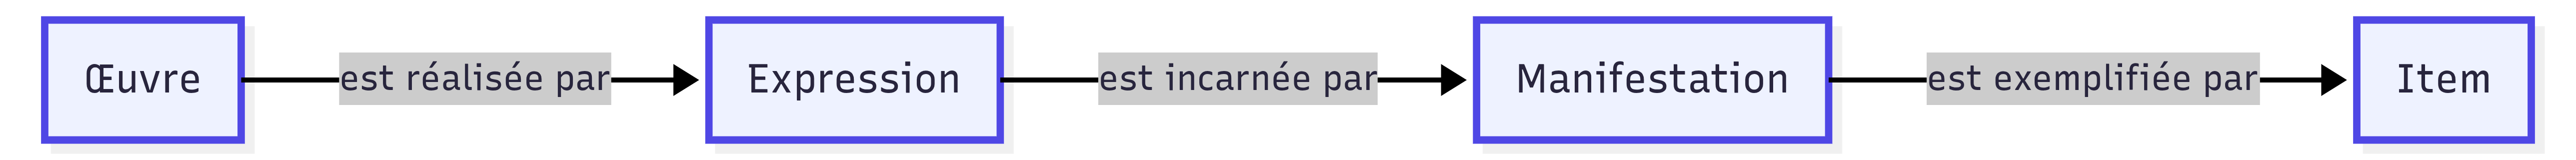
\includegraphics[width=1.0\textwidth]{images/FRBRfirstgroup.png} 
	
	\caption{Entités du modèle \gls{FRBR}} 
	
	\label{figFRBR1} 
	
\end{figure} 



Le \gls{FRBR} est qualifié de modèle entité-relation, qui modélise précisément les relations qui peuvent exister entre les différents niveaux de description et, de ce fait, entre les éléments d'un système d’information, afin de permettre à l'utilisateur de les retrouver plus facilement. Afin d’illustrer la manière dont s’articule la description d’un ouvrage bibliographique selon la modélisation proposée par le FRBR, prenons l'exemple de l'ouvrage \textit{Qu'est-ce que le cinéma} d'André Bazin. Au niveau Œuvre, est décrite l'idée intellectuelle de l'ouvrage, essentiellement matérialisée par son contexte de création. Cet ouvrage, est notamment exprimé et matérialisé au sein d'un texte intégral en quatre volumes écrit entre 1958 et 1962, dont les modalités sont décrites au niveau Expression. Cette expression de l’ouvrage est notamment publiée comme édition originale aux Editions du Cerf, dont les modalités sont décrites au niveau Manifestation. Enfin, l’exemplaire individuel de cette manifestation est potentiellement conservé dans une bibliothèque avec une côte unique, dont les caractéristiques physiques sont décrites au niveau Item. Une même œuvre peut être exprimée au sein de multiples expressions, de même qu’une expression peut faire l'objet de diverses manifestations. Le foisonnement d’éléments liés à une même œuvre peut rapidement rendre complexe la navigation de l’utilisateur au sein d’un outil de gestion des collections. La description proposée par le modèle \gls{FRBR} permet de distinguer les différentes étapes du cycle de vie d’une œuvre et ses différentes matérialisations, permettant ainsi une navigation plus fluide entre les éléments liés au sein d’un catalogue.  

Notons qu’à ces quatre entités de premier groupe Œuvre, Expression, Manifestation, Item), s'ajoutent deux entités de second groupe : Personnes et Collectivités. Elles expriment le rôle joué sur la production ou le contenu d'une ou plusieurs entités du premier groupe. \footcite{zotero-item-657} Par exemple, l'auteur est relié aux niveaux Œuvre et Expression, l'éditeur au niveau Manifestation, le catalogueur au niveau Item. 

Enfin, il existe des entités de troisième groupe intégrées au modèle, qui correspondent à des Concepts, Objets, Évènements ou Lieux liés aux entités de premier et de second groupe. \footcite{zotero-item-657} 

Réunies, les entités des trois groupes confondus modélisent une structure complexe caractérisée par les liens entre éléments, comme le montre la figure \ref{figFRBR2}  

\begin{figure}[htbp] 
	
	\centering 
	
	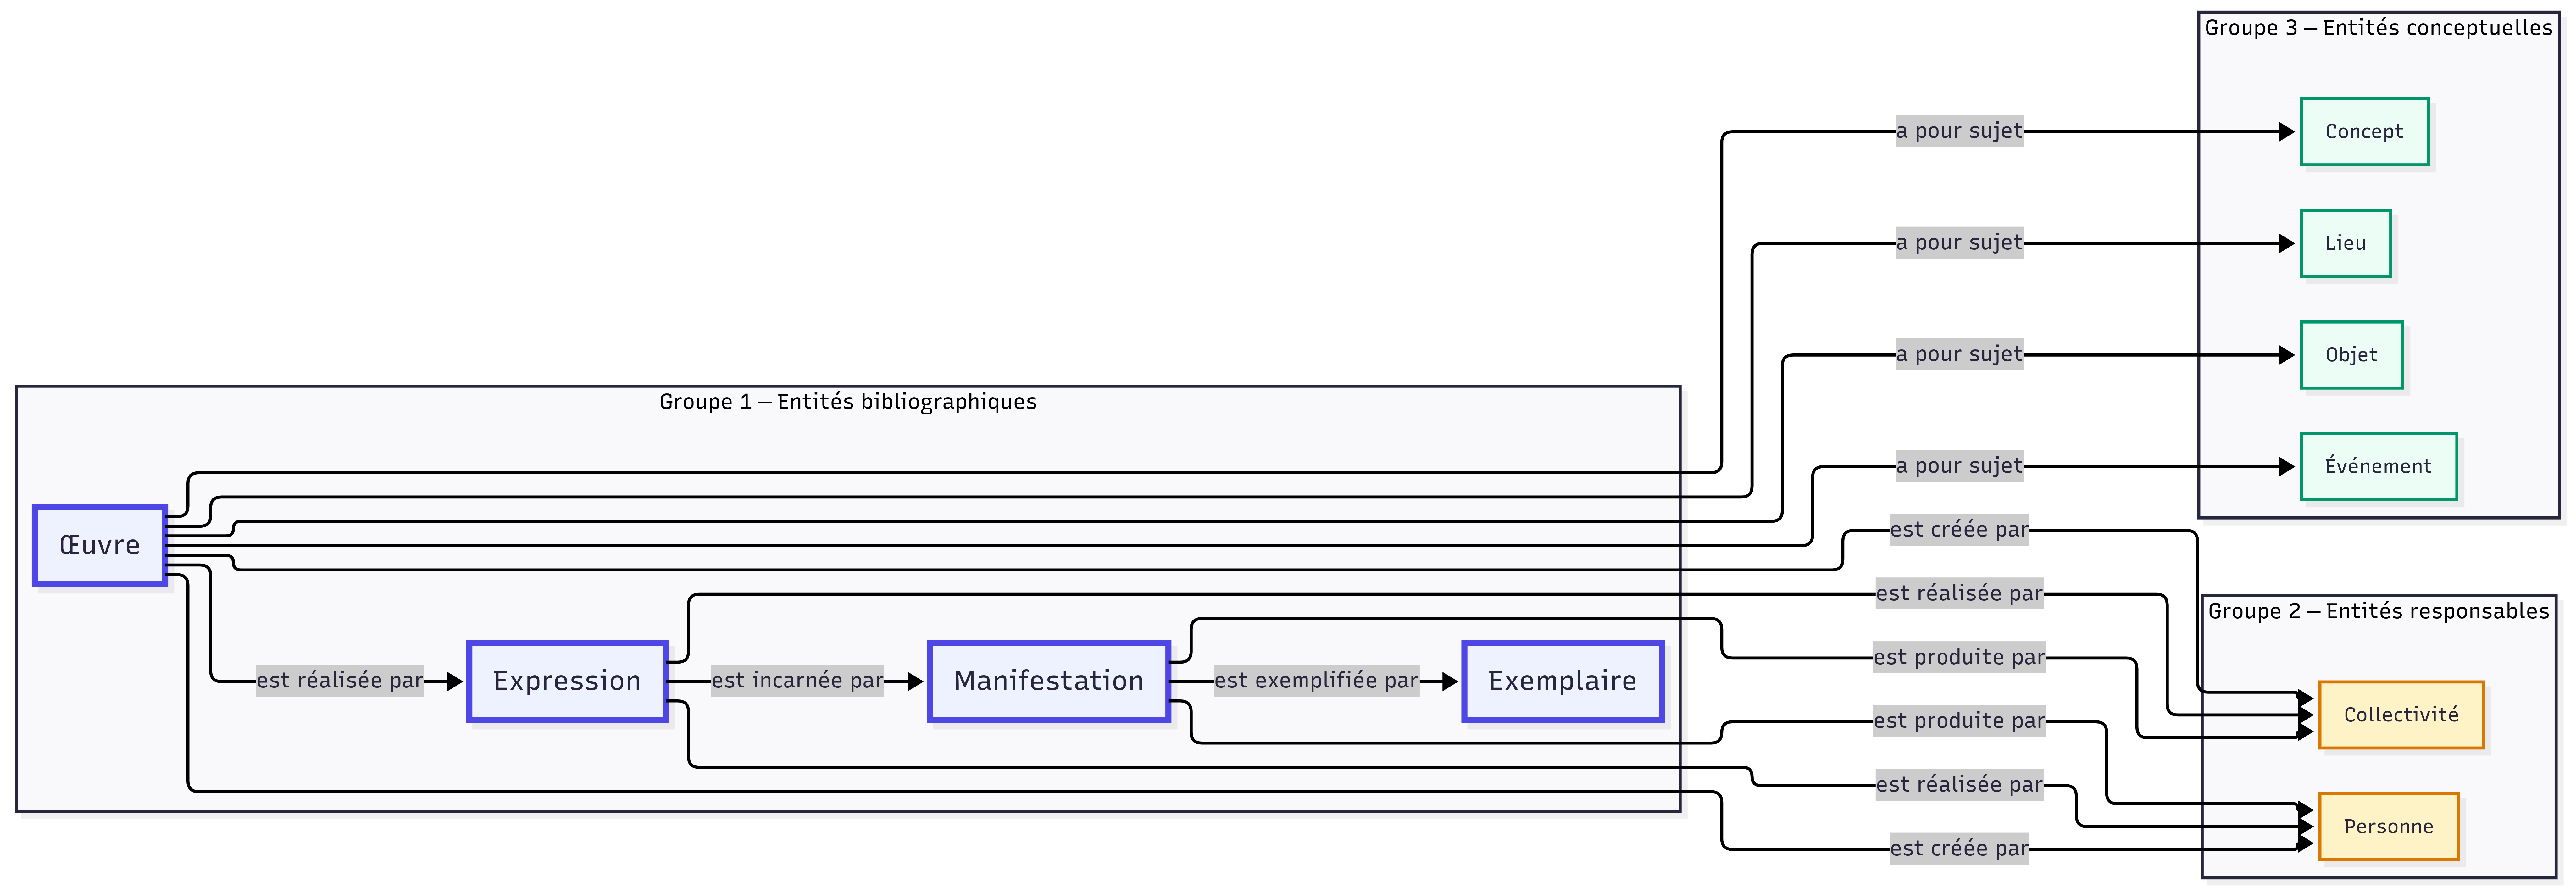
\includegraphics[width=1.0\textwidth]{images/FRBRentitesBiblio.png} 
	
	\caption{Entités du modèle FRBR} 
	
	\label{figFRBR2} 
	
\end{figure} 

Toutefois, dans le cadre de ce mémoire, nous nous concentrerons sur les entités de premier groupe, qui constituent les entités principales de description pour les archives audiovisuelles au sein du logiciel de gestion des collections créé par Skinsoft. Les entités de second et troisième groupe constituent moins des entités à part entière que des éléments de description contrôlés par des thésaurus.  

Le modèle \gls{FRBR}, fondé sur les relations entre entités, est avant tout conçu dans l’optique de faciliter la navigation de l'utilisateur au sein d'un catalogue, entre les liens qui régissent les différents éléments d'une collection.  Le \gls{FRBR} prétend en effet répondre à quatre besoins utilisateur principaux : trouver, identifier, sélectionner, obtenir. \footcite{zotero-item-653}. Il permet à l'utilisateur de localiser la ressource, d'identifier si elle correspond bien à ce qu'il cherche, de la sélectionner selon ses besoins, avant d'accéder finalement à son contenu. Nous ajouterons que le besoin fondateur de la création d'un tel modèle est également celui de pouvoir visualiser et explorer les liens de la ressource identifiée avec d'autres ressources pertinentes qui y sont directement associées. \footcite{zotero-item-653} Ce modèle de données se situerait donc à l'intersection de deux besoins principaux : celui d'améliorer la connaissance sur une ressource donnée en visibilisant ses relations, et celui d'améliorer l'expérience utilisateur en proposant une interface navigable et intuitive. 

%Donner un exemple d’institution qui utilise ce modèle et comment ça se matérialise dans un catalogue en ligne (bibliothèque kandinsky?) 

Notons que ces besoins s'appliquent non seulement à l'utilisateur faisant partie d'un public, au sein d'un catalogue ou d'une base de données en ligne, mais également à un utilisateur métier, interne à l'institution et gestionnaire des collections. C'est précisément sur les besoins métier de ce dernier que se concentre l'analyse de ce mémoire de recherche, puisque Skinsoft propose avant tout un outil de gestion des collections interne. De fait, les enjeux de l'implémentation et de l'adaptation du modèle \gls{FRBR} se situent au cœur des ambitions d'un logiciel de gestion des collections, dont l’objectif est d’améliorer l’interface afin d’assurer l’efficacité de l’utilisateur métier.  







%L'adoption de ces modèles dans les catalogues est réalisé dans l'objectif d'améliorer la visibilité des données au sein du web de données et donner accès au public aux données produites, même si ce mémoire se concentre sur l'utilisateur métier. (définir le web de données?) \footcite{zotero-item-661} 